\documentclass{article}
\usepackage[utf8]{inputenc}
\usepackage[T1]{fontenc}
\usepackage{ngerman}
\usepackage{graphicx}
 
\title{User-Centered Design\\~\\Homework 2\\ \small{T. Bento, N. Lehmann, B. Swiers}}
\date{23.04.2015}


\begin{document}

\renewcommand\abstractname{Assignment}
\maketitle


%%%%% ASSIGNMENT %%%%%
\begin{abstract}
Two parts this time:\\
\\
2.1) Learning aims: Learn about the appropriateness of user research methods during the software development process.\\
Read the following article by Christian Rohrer:\\
http://www.nngroup.com/articles/which-ux-research-methods/\\
Describe the three dimensions of user research methods named in the article.\\
What does the author say concerning the provided insights based on qualitative and quantitative research methods?\\
\\
2.2) Based on the feedback from the interview you have done in the last class revise your interview questions.\\
What changes did you make and why? Please explain.\\
Conduct at least three interviews with potential users.\\
Work together with your project team: one interviewer, other participants making notes.\\
Document the results of your interviews.
\end{abstract}

\newpage

%%%%% CONTENT %%%%%

\textit{Einzelabgabe: N. Lehmann}

\section*{2.1) Untersuchungsmethoden}

\subsection*{Dimension: Einstellung gegen Verhalten}

Die Extrema dieser Dimension stellt im Kern \textit{was Menschen sagen} und \textit{was Menschen tun} gegenüber. Welche Einstellungen ein Mensch hat spielt eine Rolle beim Verstehen seines mentalen Modells. Das mentale Modell gibt Aufschluss über eine mögliche Produktarchitektur, um der Denkweise des Benutzers zu entsprechen. Es kann eine starke Diskrepanz zwischen Einstellung und Verhalten geben.
\begin{itemize}
\item Einstellungsorientierte Methoden
\begin{itemize}
\item Card Sorting
\item Surveys
\end{itemize}

\item Verhaltensorientierte Methoden
\begin{itemize}
\item A/B Testing
\item Eyetracking
\end{itemize}

\item hybride Formen
\begin{itemize}
\item Usabiliy studies
\item Field studies
\end{itemize}
\end{itemize}

\subsection*{Dimension: qualitativ gegen quantitativ}

\begin{itemize}
\item Qualitative Methoden\\
Eignen sich gut um Fragen, wie \textit{Warum ... ?} oder \textit{Wie löst man das Problem ... ?} zu beantworten und können direkt gesammelt werden, z.B. durch Beobachtung.
\item Quantitative Methoden\\
Eignen sich gut um Fragen, wie \textit{Wie viel ... ?} oder \textit{Wie viele ... ?} zu beantworten und können indirekt gesammelt werden. Häufig werden statistische, analytische Werkzeuge eingesetzt, um die Daten zu erheben.
\end{itemize}
\newpage

\subsection*{Die beiden Dimensionen gegeneinander}
Verwendete Methoden korrelieren mit beiden Dimensionen und können (wie im Bild unten gezeigt) entlang den Dimensionen abgebildet werden.\\
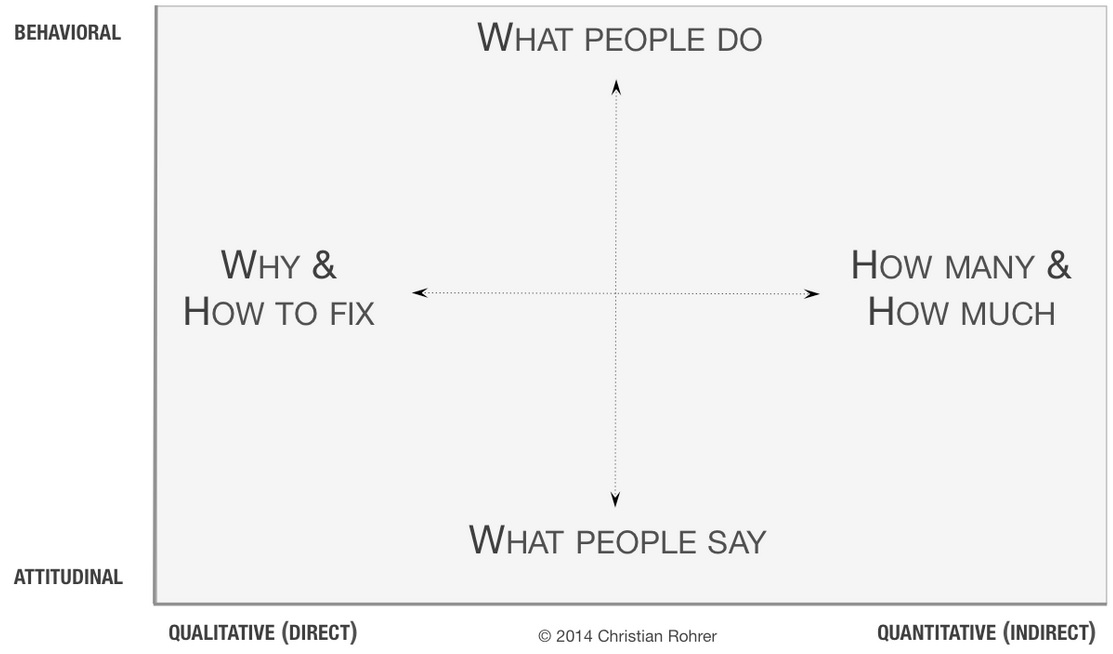
\includegraphics[width=12cm]{methoddim.jpg}

\subsection*{Dimension: Verwendungskontext}

Der Verwendungskontext von Methoden wird in 4 Bereiche klassifiziert:
\begin{itemize}
\item \textbf{natürliche Verwendung}\\
Die natürliche Verwendung versucht den Untersuchungsgegenstand im natürlichen Kontext (Alltag) zu untersuchen. Einstellungen und Verhalten werden unter realistischen Umständen (unkontrolliert) untersucht. Diese Art der Untersuchung ermöglicht eine hohe äußere Gültigkeit, erzeugt allerdings auch den Effekt, dass das Untersuchungsergebnis sehr offen wird.  
\item \textbf{angeleitete Verwendung}\\
Die angeleitete Verwendung untersucht spezielle Aspekte des Untersuchungsgegenstandes um weitergehende Einsichten zu gewinnen. Der Grad der Kontrolle kann je nach Studienziel variieren.
\item \textbf{keine Verwendung}\\
Untersuchungen dieser Art richten sich auf breiter aufgestellte Studien, wie soziokulturelle Untersuchungen. 
\item \textbf{hybride Verwendung}\\
Hier kommen kreative Methoden, wie Partizipativ-Design oder Konzepttests, zum Einsatz.
\end{itemize}

\subsection*{Was sagt der Autor über die Einblicke auf Basis von qualitativer und quantitativer Forschung?}

\begin{itemize}
\item Qualitative Forschung\\
Eignet sich gut um Fragen, wie \textit{Warum ... ?} oder \textit{Wie löst man das Problem ... ?} zu beantworten. Die Ergebnisse dieser Forschung liefern Gründe warum etwas so ist wie es ist und ermöglicht das elementare Beseitigen von (Prozess-)Fehlern.
\item Quantitative Forschung\\
Eignet sich gut um Fragen, wie \textit{Wie viel ... ?} oder \textit{Wie viele ... ?} zu beantworten. Durch Ergebnisse dieser Forschung wird klar, welche Probleme den größten Einfluss haben und auf welche Funktionen man sich konzentrieren sollte.
\end{itemize}

\newpage

\textit{Gruppenabgabe}

\section*{2.2) Interviews}

\subsection*{Änderungen}

\begin{itemize}
\item Wir haben die Anrede von der Sie-Form zur Du-Form geändert, um einen persönlicheren Kontakt zur Zielgruppe zu erlangen.
\item Wir haben alle geschlossenen Fragen eliminiert und in offene Fragen transformiert.
\item Wir haben Fachbegriffe und Abkürzungen eliminiert, die unverständlich sein könnten, bzw. geändert in verständlichere Sprache.
\end{itemize}


\subsection*{Fragebogen}

\begin{enumerate}
\item Welches Fach (nach welcher Studienordnung) studierst Du und warum?
\begin{itemize}
\item Informatik
\item Bioinformatik
\item wusste nicht, was er/sie nach dem Abi tun sollte
\item Berufsberatung ergab etwas mit IT, also Informatik
\item Abiturnote war schlecht (2,5): Ich konnte mich nicht auf die Fächer bewerben, auf die ich Lust hatte.
\item Interesse
\item Brauche es für die Arbeit, habe mich dagegen gestreubt.
\item Reine Biologie ist mir zu langweilig und ich will in die Forschung.
\item Weil ich schon eine Ausbildung gemacht habe und die Inhalte vertiefen will.
\item Weil ich zu faul war für das Maschinenbaustudium.
\end{itemize}

\item Wie sieht Dein Alltag an einem Universitätstag aus?
\begin{itemize}
\item Besuch der Vorlesung, Essen in der Mensa, Tutorium, zu Hause Übungsaufgaben lösen
\item um 8 Uhr in der Universität zur Vorlesung und Übung, mit Übungspartner treffen und Übungen bearbeiten, zu Hause lernen oder Arbeiten gehen
\item Von 10 bis 14 Uhr Universität, zu Hause Pause und Übungsaufgaben am Rechner, Papiere lesen oder Reviews schreiben, abends Sport oder Computer spielen
\item Vorlesungen, Tutorien, zwischendurch setze ich mich mit Kommilitonen zusammen
\item Zeit in der Universität: von 10 Uhr bis 19 Uhr
\end{itemize}

\item Welche Lernverwaltungssoftware (LMS) der Freien Universität Berlin hast Du schon einmal verwendet?
\begin{itemize}
\item KVV / Sakai CLE
\item Campus Management (CM)
\item Blackboard
\end{itemize}

\item Wann und wo verwendest Du die Lernverwaltungssoftware der Freien Universität Berlin?
\begin{itemize}
\item Sakai CLE (KVV)
\begin{itemize}
\item in der Universität, wenn ich einen Übungszettel benötige
\item in der Universität, in einer Vorlesung für das Skript (Skript, wird nicht gespeichert)
\item zu Hause, zum Lösen eines Übungszettels
\item Überall wo ich WLAN habe, weil ich ständig nachgucke, ob es etwas Neues gibt.
\end{itemize}
\item Campus Management (CM)
\begin{itemize}
\item in der Universität, um sich am Anfang des Semesters für ein Modul anzumelden
\item zu Hause, um sich am Anfang des Semesters für ein Modul anzumelden
\end{itemize}
\item Blackboard (BB)
\begin{itemize}
\item zu Hause, aber nur wenn es nicht anders geht
\item in der Universität, einige Dozierende verwenden kein KVV
\end{itemize}
\end{itemize}

\item Wie zufrieden bist Du im Allgemeinen zur Zeit mit der derzeitigen Lernverwaltungssoftware der Freien Universität Berlin und warum? (Bewertung je System)
\begin{itemize}
\item Allgemein
\begin{itemize}
\item Negativ: Es gibt zu viele verschiedene Systeme, besser wäre ein System.
\item Ich bin zufrieden weil es läuft wie es laufen soll.
\end{itemize}
\item Sakai CLE (KVV)
\begin{itemize}
\item Negativ ist, dass man sich immer wieder neu einloggen muss, da man nach einiger Zeit automatisch ausgeloggt wird.
\item einfach zu bedienen, ich weiß nicht was andere Leute daran kritisieren
\item Im Großen und Ganzen sehr gut, weil das System sehr übersichtlich ist.
\item Anmeldung zu einem Tutorium ist sehr einfach (point \& klick)
\item gut nach Fächern strukturiert
\item Gut, man findet was man sucht und wird per Email informiert.
\item Zufrieden, aber es ist Luft nach oben: die Übersicht ist gut, ich wünsche mir aber mehr Automatisierungsmöglichkeiten um Inhalte auf meine Geräte zu synchronisieren.
\item Übersetzung Deutsch/Englisch ist schlecht
\item überall wo ich Internet habe, komme ich an die Sachen ran
\item Workspace nutze ich nicht
\end{itemize}
\item Campus Management (CM)
\begin{itemize}
\item Negativ, die Noteneintragung dauert lange.
\item Apple-User haben ein Problem mit diesem System
\end{itemize}
\item Blackboard (BB)
\begin{itemize}
\item Schlechtestes System: viele Funktionen funktionieren nicht, es ist sehr unübersichtlich, zu Kursen anmelden ist sehr umständlich
\end{itemize}
\end{itemize}

\item Welche Funktionen der LMS verwendest Du wirklich?
\begin{itemize}
\item Sakai CLE (KVV)
\begin{itemize}
\item Übungszettel ansehen/herunterladen
\item Übungszettel abgeben/hochladen
\item Anmeldung zu einem Tutorium
\item Skripte/Folien/Materialien ansehen/herunterladen
\item Ankündigungen
\item Forum (inhaltliche und organisatorische Fragen stellen)
\item Punkte/Noten einsehen
\item Herausfinden wo mein Raum ist
\end{itemize}
\item Campus Management (CM)
\begin{itemize}
\item Anmeldung zu Modulen
\end{itemize}
\item Blackboard (BB)
\begin{itemize}
\item Übungszettel ansehen/herunterladen
\item Übungszettel abgeben/hochladen
\item Skripte/Folien/Materialien ansehen/herunterladen
\item Forum (inhaltliche und organisatorische Fragen stellen)
\end{itemize}
\end{itemize}

\item Wie zufrieden bist Du mit den genannten Funktionen und warum?
\begin{itemize}
\item Sakai CLE (KVV)
\begin{itemize}
\item Übungszettel ansehen/herunterladen: Sache von 2 Klicks, benachrichtigt werden ist gut, sehr zufrieden
\item Übungszettel abgeben/hochladen: einfach, man kann kommentieren, wenn was fehlt ist kommentieren super, Feedback kann man geben, sehr zufrieden
\item Anmeldung zu einem Tutorium: sehr simpel, also sehr gut
\item Skripte/Folien/Materialien ansehen/herunterladen: Ordnerstruktur ist sehr übersichtlich, aber ich hatte keine Möglichkeit den ganzen Ordner herunterzuladen oder mit meinen Geräten zu synchronisieren, das hat mich gestört
\item Ankündigungen
\item Forum (inhaltliche und organisatorische Fragen stellen): mit anderen Studenten in Kontakt kommen, es wurde immer geantwortet, ist gut strukturiert, positiv
\item Punkte/Noten einsehen
\item Herausfinden wo mein Raum ist
\item Kalender: Ich wünsche mir, dass die Dozenten mehr Gebrauch davon machen, wenn ich mich in mein Tutorium anmelde sollte das auch in meinem Kalender auftauchen, sollte mit anderen Kalendern synchronisierbar sein
\end{itemize}
\item Campus Management (CM)
\begin{itemize}
\item Anmeldung zu Modulen: Man findet die Kurse nicht oder sie heißen anders, das ist schlecht!
\end{itemize}
\end{itemize}

\item Was würdest Du anders machen?
\begin{itemize}
\item Keine Ahnung!
\item Ich würde das KVV als App herausbringen, das wäre ein viel leichterer Zugriff.
\item Alle Systeme sollten zu einem System werden, doppelte Arbeit.
\item Das KVV ist optimal, das CM benutzen ist stressig.
\item die Übersetzung
\item KVV stürzt manchmal ab
\item Ich habe keine Lust mich damit auseinander zu setzen.
\item ich glaube Dozenten haben keine Lust sich damit auseinander zu setzen.
\item Die meisten Probleme, die ich habe, sind nicht durch Software lösbar.
\item Im CM das Suchproblem ändern/lösen.
\item Ressources Ordner sollte downloadbar/synchronisierbar sein
\item KVV: Beim Gradebook werden dinge angezeigt, die mich nicht betreffen.
\item KVV: Die Home-Übersicht erschlägt einen, hier braucht man nur den Kalender, Meldungen aber keine Informationen über irgendwelche Bereiche.
\item Eine automatisierte Übungszettel-Downloadgeschichte wäre eine schöne Lösung.
\end{itemize}

\item Verwendest Du zum Erreichen Deiner studienbezogenen Ziele auch andere Softwaresysteme oder Webseiten, etc.? Wenn ja, welche und warum?
\begin{itemize}
\item Debian
\item GetIt
\item keine weitere Software
\item Youtube (viel)
\item MOOC (massiv online open courses)
\item Webseiten, die mit Videos einfach erklären wie etwas funktioniert
\item Eclipse
\item Sublime Editor
\item Open Office
\item Latex
\item Wolfram Alpha
\item Matheforum Matheplanet
\item Foren zum Programmieren
\item Java Bibliothek
\item in einer kleinen Gruppe Aufgaben durchsprechen ist wichtiger als Software
\item Android-Entwicklungsumgebung
\item Galileo Open Books
\item kostenlose Softwarebücher im Internet
\item Wikipedia
\item gitlab von der Universität um meine Übungen über meine Geräte zu synchronisieren
\item ssh um auf Unix-Systemen zu arbeiten
\end{itemize}

\item Auf welchen Endgeräten verwendest Du die von Ihnen bevorzugte Software?
\begin{itemize}
\item Poolrechner
\item Python auf dem iPad
\item Smartphone
\item Laptop (oft MacBook)
\item Tablet (Linux, Android, iPad, wenig genutzt)
\item Workstation (PC)
\end{itemize}

\item Welche Probleme während Deines derzeitigen Studienalltags werden durch Software nicht gelöst oder können Deiner Meinung nach nicht von Software gelöst werden?
\begin{itemize}
\item Keine Ahnung!
\item Kontaktaustausch mit den Tutoren kann man ja machen.
\item Zeitmanagement kann man auch übers Smartphone machen.
\item Planung, Stundenplan, rechtzeitig eintragen
\item Übungszettel werden zu spät hochgeladen, aber Abgabetermine bleiben gleich.
\item nach der Veröffentlichung eines Übungszettels wird der Übungszettel geändert, aber man kriegt das nicht mit und gibt eine Lösung zur alten Version ab
\item man braucht länger, um mit Software zu lernen, mit Menschen reden ist wichtig
\item Verständnisfragen kann man nicht mit Software lösen
\item Leistungsdruck, bestimmte Regelung, wie viel man schaffen muss
\item die Bewertung was man gelernt hat, weil jeder anders lernt
\item sehr spezielle Beweisführungen, bei denen man keine konkreten Beispiele findet, gerade in Mathe
\item Wo finde ich Inhalte?
\item Das Einstellen der biologischen Uhr: einen guten Wochen-Rhythmus finden
\item Übungsaufgaben verstehen ist das Schwierigste
\item Schlafmangel ist wichtiger Faktor
\end{itemize}

\item Wer unterstützt Dich während Deines Studiums und wie?
\begin{itemize}
\item Studierende aus dem höheren Semester helfen bei Fragen
\item Tutoren helfen bei Fragen
\item Lerngruppen!
\item Mitstudenten, bei Programmierproblemen
\item Mentoren, wenn man Fragen hat wie man das Studium ausrichten soll
\item Kollegen bei kurzen Fragen
\item Motivation durch Freunde und Eltern
\item sich kennen lernen ist wichtig
\item Eltern und Bafög mit Geld
\end{itemize}

\item Wenn Du eine Empfehlung zu einem Modul oder einer Lehrveranstaltung erhalten, was sind für Dich die wichtigsten Punkte?
\begin{itemize}
\item interessiert es mich
\item muss ich es machen
\item meinem Semester entsprechend: Wenn die Person die mir das empfiehlt es im 4. Semester gemacht hat und es mir fürs 2. Semester empfiehlt, dann zweifel ich an der Empfehlung, weil er es selber nicht so gemacht hat. Ich würde auch gucken wie gut er damit zurecht gekommen ist.
\item es ist nicht so wichtig wie viele Leute mir das empfehlen sondern wer
\item wenn ich Unterstützung von guten Leuten bekomme, versuche ich auch schwierige Module
\item zeitlich, ob es in meinen Plan passt
\item ob es einfach ist, wie viel ich investieren muss
\item LP
\item praktische Module sind besser, theoretische Module sind langweilig
\item Verständlichkeit: wie verständlich bringt der Dozent die Inhalte rüber, wie nah ist er an den Studierenden
\item inhaltlich interessant
\item wer macht das Modul / die Lehrveranstaltung auch (Studierende)
\item ist der Prof gut (die Art wie man unterrichtet ist entscheidend)
\item die Person, die mir das Modul empfiehlt, muss das Modul belegt haben
\item Inhalte sind wichtiger
\item praktisch / theoretisch ist wichtig
\item praktisch / theoretisch ist eher unwichtig
\item sind die Vorlesungen ansprechend
\item Welcher Tutor ist in der LV?
\end{itemize}

\item Wie schätzt Du Deine Studienleistungen ein?
\begin{itemize}
\item ich bin zufrieden mit mir, weil ich viel Zeit darin investiere
\item ich bin in der Regelstudienzeit, ich bin zufrieden
\item schlecht, weil ich habe kaum etwas bestanden, andere Dinge waren mir wichtiger
\item gut
\item inzwischen relativ gut
\item besser, kein Überflieger, aber vom Stand her höher
\item ich wünsche mir manchmal mehr zu machen, ich frage mich aber, ob das sinnvoll ist
\item ich hoffe, das Level so halten zu können
\end{itemize}
\end{enumerate}

\end{document}